\documentclass[11pt]{article}

\usepackage[letterpaper,margin=1in]{geometry}
\usepackage[T1]{fontenc}
\usepackage{lmodern}
\usepackage{microtype}
\usepackage{amsmath,amssymb,mathtools}
\usepackage{booktabs}
\usepackage{graphicx}
\usepackage{float}
\usepackage{xcolor}
\usepackage{enumitem}
\usepackage{fancyhdr}
\usepackage{hyperref}
\usepackage{caption}
\usepackage{subcaption}

\definecolor{navy}{HTML}{17365D}
\definecolor{muted}{HTML}{5B6573}
\definecolor{lightblue}{HTML}{EEF3F8}
\hypersetup{colorlinks=true,linkcolor=navy,citecolor=navy,urlcolor=navy,
  pdftitle={Reproducing Explainable Regime-Aware Investing},
  pdfauthor={Manuel T.}}
\setlist{nosep,leftmargin=1.5em}
\captionsetup{font=small,labelfont=bf}
\graphicspath{{../figures/}}
% Generated from results.json by make_latex_numbers.py; do not edit.
\newcommand{\PubHMMSharpe}{2.18}
\newcommand{\PubHMMMaxDD}{-5.43\%}
\newcommand{\RepHMMSharpe}{1.59}
\newcommand{\RepHMMMaxDD}{-9.35\%}
\newcommand{\RepHMMReturn}{53.17\%}
\newcommand{\RepHMMVol}{10.23\%}
\newcommand{\PubHMMTurnover}{0.0079}
\newcommand{\RepHMMTurnover}{0.0166}
\newcommand{\RepHMMTurnoverQ}{0.0707}
\newcommand{\PubKNNSharpe}{1.81}
\newcommand{\PubKNNMaxDD}{-12.52\%}
\newcommand{\RepKNNSharpe}{0.79}
\newcommand{\RepKNNMaxDD}{-13.20\%}
\newcommand{\RepKNNReturn}{33.66\%}
\newcommand{\RepKNNVol}{14.91\%}
\newcommand{\PubKNNTurnover}{0.5665}
\newcommand{\RepKNNTurnover}{0.4949}
\newcommand{\RepKNNTurnoverQ}{1.0000}
\newcommand{\PubEqualSharpe}{1.59}
\newcommand{\PubEqualMaxDD}{-9.87\%}
\newcommand{\RepEqualSharpe}{1.68}
\newcommand{\RepEqualMaxDD}{-7.96\%}
\newcommand{\RepEqualReturn}{47.98\%}
\newcommand{\RepEqualVol}{8.88\%}
\newcommand{\PubSPXSharpe}{1.18}
\newcommand{\PubSPXMaxDD}{-14.62\%}
\newcommand{\RepSPXSharpe}{1.36}
\newcommand{\RepSPXMaxDD}{-18.76\%}
\newcommand{\RepSPXReturn}{69.38\%}
\newcommand{\RepSPXVol}{15.22\%}
\newcommand{\RepHMMNetSharpe}{1.57}
\newcommand{\RepHMMNetMaxDD}{-9.40\%}
\newcommand{\RepHMMNetReturn}{52.31\%}
\newcommand{\RepKNNNetSharpe}{0.38}
\newcommand{\RepKNNNetMaxDD}{-20.70\%}
\newcommand{\RepKNNNetReturn}{12.91\%}
\newcommand{\PriceStart}{2007-03-01}
\newcommand{\PriceEnd}{2026-02-20}
\newcommand{\OOSStart}{2023-06-02}
\newcommand{\OOSEnd}{2026-02-20}
\newcommand{\OOSObs}{682}
\newcommand{\VolWindow}{60}
\newcommand{\MomWindow}{20}
\newcommand{\TemplateCount}{6}
\newcommand{\ValidationDays}{126}
\newcommand{\RefitFrequency}{10}
\newcommand{\OrderFrequency}{63}
\newcommand{\KNNNeighbors}{50}
\newcommand{\RiskAversion}{3.0}
\newcommand{\TurnoverPenalty}{0.0001}
\newcommand{\MaxWeight}{60\%}
\newcommand{\RealizedCost}{5}
\newcommand{\RandomSeed}{7}
\newcommand{\CandidateStates}{2--6}
\newcommand{\HMMSharpeGap}{-0.59}
\newcommand{\HMMDDGap}{-3.92\%}
\newcommand{\TurnoverRatio}{29.9}
\newcommand{\AvgSPYWeight}{44.58\%}
\newcommand{\AvgTLTWeight}{22.81\%}
\newcommand{\AvgGLDWeight}{25.08\%}
\newcommand{\AvgUSOWeight}{2.40\%}
\newcommand{\AvgUUPWeight}{5.14\%}


\pagestyle{fancy}
\fancyhf{}
\fancyhead[L]{\small Reproducing Explainable Regime-Aware Investing}
\fancyhead[R]{\small Reproducibility audit}
\fancyfoot[C]{\thepage}
\setlength{\headheight}{14pt}

\title{\textbf{Reproducing Explainable Regime-Aware Investing}\\
\large A Independent Implementation and Reproducibility Audit}
\author{Manuel T.\thanks{AI assistance was used in creating this document.}}
\date{September 2026}

\begin{document}
\maketitle

\begin{abstract}
We present a reproduction of the Wasserstein hidden Markov model (HMM) allocation framework proposed in \emph{Explainable Regime Aware Investing}. The disclosed architecture combines causal market-state features, expanding-window Gaussian HMM estimation, predictive model-order selection, persistent regime templates matched by Gaussian 2-Wasserstein distance, and transaction-penalized mean--variance optimization. We implement each element under explicit assumptions and compare the resulting out-of-sample record with the paper's published targets. The reproduction obtains a gross Sharpe ratio of \RepHMMSharpe{} and maximum drawdown of \RepHMMMaxDD{}, versus published values of \PubHMMSharpe{} and \PubHMMMaxDD{}. Equal weight achieves a reproduced Sharpe of \RepEqualSharpe{}, so the headline claim of superior risk-adjusted performance is not verified. The qualitative stability result is stronger: average one-way turnover is \RepHMMTurnover{} for the HMM and \RepKNNTurnover{} for the K-nearest-neighbor (KNN) comparator, a \TurnoverRatio{}-fold difference. Exact numerical reproduction is impossible from the publication because essential instruments, hyperparameters, transformations, and return conventions are omitted, while the submitted source contains conflicting result tables. The exercise therefore reproduces the method, but not the headline empirical claims.
\end{abstract}

\noindent\textbf{Keywords:} regime switching, hidden Markov model, Wasserstein distance, portfolio allocation, reproducibility, transaction costs.\\
\textbf{JEL classification:} C22, C52, C58, G11.

\section{Introduction}

Regime-aware allocation seeks to condition portfolio decisions on latent market states rather than assume a single stationary return distribution. The approach is economically appealing: correlations, volatility, and expected returns can change abruptly, while a latent-state model can compress those changes into an interpretable probability vector. The implementation problem is equally important. A rolling HMM can change its selected number of states, permute state labels after refitting, and transmit noisy conditional moments into an unstable optimizer.

Boukardagha \cite{boukardagha2026} proposes a Wasserstein HMM intended to address these problems. Model order is selected by predictive likelihood, Gaussian components are mapped to persistent templates using the 2-Wasserstein metric, and template probabilities feed a transaction-cost-aware mean--variance optimizer. The paper reports an HMM Sharpe ratio of \PubHMMSharpe{}, compared with \PubEqualSharpe{} for equal weight and \PubSPXSharpe{} for an SPX benchmark. It also reports materially lower HMM turnover than a KNN conditional-moment estimator.

The contribution of this paper is not another tuned variant. It is a replication with three goals:

\begin{enumerate}
  \item implement the disclosed causal architecture without access to the author's code;
  \item separate explicit assumptions from information actually reported in the source paper; and
  \item identify which qualitative and quantitative claims survive under a reasonable, fully auditable specification.
\end{enumerate}

The conclusion is mixed. The HMM is far more stable than the KNN baseline, but it does not reproduce the published Sharpe or drawdown and does not outperform equal weight in our sample. This distinction matters: architectural plausibility is not the same as empirical verification.

\section{Target Study and Replication Questions}

The target study evaluates five economic sleeves labeled SPX, BOND, GOLD, OIL, and USD using Yahoo Finance adjusted closes. It builds a daily feature vector from returns, rolling volatility, and rolling momentum; estimates a variable-order Gaussian HMM; stabilizes component identities with Wasserstein templates; and performs constrained mean--variance allocation. A non-parametric KNN estimator and two passive portfolios serve as comparators.

We organize the audit around four questions:

\begin{description}[style=nextline]
  \item[RQ1: Implementability.] Is the published architecture sufficiently clear to produce a strictly causal working system?
  \item[RQ2: Numerical reproducibility.] Do reasonable explicit choices recover the published risk-adjusted performance and drawdown?
  \item[RQ3: Stability.] Does template-based parametric inference materially reduce turnover relative to KNN?
  \item[RQ4: Identification.] Which missing choices prevent a unique mapping from the paper to executable code?
\end{description}

\section{Methodology}

\subsection{Causal feature construction}

Let \(P_t\in\mathbb{R}_{+}^{N}\) denote adjusted closing prices and let
\begin{equation}
  r_t = \log P_t - \log P_{t-1}
  \label{eq:returns}
\end{equation}
be the vector of log returns. To resolve the source paper's timing ambiguity, the decision for session \(t\) uses a lagged feature vector
\begin{equation}
  x_t = \begin{bmatrix}r_{t-1} & \sigma_{t-1}^{(\VolWindow)} & m_{t-1}^{(\MomWindow)}\end{bmatrix}^{\!\top},
  \label{eq:features}
\end{equation}
where \(\sigma_{t-1}^{(\VolWindow)}\) is componentwise rolling volatility over \VolWindow{} sessions and \(m_{t-1}^{(\MomWindow)}\) is componentwise mean return over \MomWindow{} sessions. This construction makes the information set explicit: \(x_t\) contains no close or return from session \(t\).

\subsection{Predictive Gaussian HMM}

Conditional on state \(z_t=k\), standardized features follow
\begin{equation}
  x_t\mid z_t=k \sim \mathcal{N}(a_k,B_k), \qquad
  \Pr(z_t=j\mid z_{t-1}=i)=A_{ij}.
  \label{eq:hmm}
\end{equation}
Candidate orders range from \CandidateStates{} states. On an order-selection date, a model is fitted to the expanding history preceding a trailing validation block of \ValidationDays{} observations. For candidate order \(K\), the score is
\begin{equation}
  S_t(K)=\frac{1}{|V_t|}\log p(X_{V_t}\mid X_{H_t\setminus V_t},K)-\lambda_K q(K),
  \label{eq:selection}
\end{equation}
where \(q(K)\) counts free mean, covariance, and transition parameters. The maximizing order is retained until the next selection date. The HMM is re-estimated every \RefitFrequency{} sessions and order is reconsidered every \OrderFrequency{} sessions.

\subsection{Persistent Wasserstein templates}

Repeated HMM estimation leaves component labels unidentified. Consider two Gaussian components with parameter pairs \((a_1,B_1)\) and \((a_2,B_2)\). Their squared 2-Wasserstein distance is
\begin{equation}
\begin{split}
 W_2^2 &= \|a_1-a_2\|_2^2 \\
 &\quad + \operatorname{tr}\!\left(B_1+B_2-2\left(B_2^{1/2}B_1B_2^{1/2}\right)^{1/2}\right).
\end{split}
\label{eq:wasserstein}
\end{equation}
Each newly estimated component is mapped to the nearest of \TemplateCount{} persistent templates. Template parameters are updated by exponential smoothing. Multiple components may map to one template, which allows the active HMM order to differ from the fixed identity vocabulary.

\subsection{From feature states to return moments}

The source paper denotes both HMM feature moments and portfolio return moments by \(\mu\) and \(\Sigma\), although the feature vector has dimension \(3N\) and portfolio weights have dimension \(N\). A projection is therefore necessary but unspecified. Our bridge is posterior-weighted estimation of next-session asset-return moments. For state \(k\),
\begin{equation}
  \widehat\mu_k=\frac{\sum_{s<t}\xi_{s,k}R_s}{\sum_{s<t}\xi_{s,k}},
  \qquad
  \widehat\Sigma_k=\operatorname{ShrinkCov}\!\left(\{R_s,\xi_{s,k}\}_{s<t}\right),
  \label{eq:returnmoments}
\end{equation}
where \(\xi_{s,k}=\Pr(z_s=k\mid X_{1:s})\). Covariances are shrunk toward their diagonal following the motivation of Ledoit and Wolf \cite{ledoitwolf2004}. Component return moments inherit the template mapping and are exponentially smoothed with their templates.

If \(p_{t,g}\) is the filtered probability of template \(g\), allocation inputs are
\begin{equation}
  \widehat\mu_t=\sum_{g=1}^{G}p_{t,g}\widehat\mu_g,
  \qquad
  \widehat\Sigma_t=\sum_{g=1}^{G}p_{t,g}\widehat\Sigma_g.
  \label{eq:mixture}
\end{equation}
We follow the target paper's displayed equation and do not add the between-template covariance term that would appear in an exact Gaussian mixture covariance.

\subsection{Portfolio optimization}

The daily portfolio solves
\begin{equation}
\begin{aligned}
\max_{w_t}\quad & \widehat\mu_t^\top w_t
 - \gamma w_t^\top\widehat\Sigma_t w_t
 - \tau\|w_t-w_{t-1}\|_1 \\
\text{s.t.}\quad & \mathbf{1}^\top w_t=1,\quad 0\le w_{t,i}\le w_{\max}.
\end{aligned}
\label{eq:mvo}
\end{equation}
We set \(\gamma=\RiskAversion{}\), \(\tau=\TurnoverPenalty{}\), and \(w_{\max}=\MaxWeight{}\). The \(L^1\) term is solved through an exact linear epigraph rather than a smooth approximation. One-way turnover is
\begin{equation}
  \mathrm{TO}_t=\frac{1}{2}\|w_t-w_{t-1}\|_1.
  \label{eq:turnover}
\end{equation}

\subsection{KNN comparator}

The KNN baseline standardizes the same causal feature history, selects the \KNNNeighbors{} nearest prior states in Euclidean distance, computes their mean return and Ledoit--Wolf covariance, and applies the identical optimizer. This comparator isolates the stability imparted by the parametric state model and persistent templates.

\section{Data and Experimental Protocol}

The paper provides economic labels rather than exact Yahoo symbols. We map SPX to SPY, BOND to TLT, GOLD to GLD, OIL to USO, and USD to UUP. These are investable U.S.-listed ETF proxies with adjusted closes. Because UUP is the last series to begin, the complete common panel runs from \PriceStart{} through \PriceEnd{}, despite the target study describing a nominal start in 2005.

The out-of-sample interval is \OOSStart{} through \OOSEnd{} and contains \OOSObs{} sessions. This date range is reverse-engineered from the target figures and the observation counts implied by its regime and allocation tables. The HMM and KNN always train on observations strictly earlier than the return being realized. All random initialization uses seed \RandomSeed{}.

Primary comparisons use gross returns because the target paper includes a turnover penalty in optimization but does not separately state whether performance tables subtract realized trading costs. We additionally report net returns after \RealizedCost{} basis points per unit of one-way turnover. Sharpe ratios are annualized from daily arithmetic returns with zero risk-free rate, and maximum drawdown is calculated from compounded wealth.

\begin{table}[H]
\centering
\caption{Key assumptions required by omitted implementation details.}
\label{tab:assumptions}
\begin{tabular}{p{0.34\linewidth}p{0.55\linewidth}}
\toprule
Item & Replication choice \\
\midrule
Tradable proxies & SPY, TLT, GLD, USO, UUP adjusted closes \\
Feature timing & Lagged one session; no session-\(t\) information in \(w_t\) \\
HMM covariance & Full covariance in standardized feature space \\
Candidate order & \CandidateStates{} states \\
Persistent identities & \TemplateCount{} templates, nearest Wasserstein mapping \\
Refit / order cadence & Every \RefitFrequency{} / \OrderFrequency{} sessions \\
Optimizer & Long-only, fully invested, \MaxWeight{} cap \\
Costs & Gross primary record; \RealizedCost{} bps sensitivity \\
\bottomrule
\end{tabular}
\end{table}

\section{Results}

\subsection{Published targets versus reproduced outcomes}

Table~\ref{tab:mainresults} gives the central result. The reproduced HMM Sharpe is \RepHMMSharpe{}, a gap of \HMMSharpeGap{} relative to the published \PubHMMSharpe{}. Its maximum drawdown is \RepHMMMaxDD{}, compared with the published \PubHMMMaxDD{}. The reproduction therefore does not verify the headline quantitative result. Moreover, the reproduced equal-weight portfolio attains a Sharpe of \RepEqualSharpe{} and a maximum drawdown of \RepEqualMaxDD{}, outperforming the reproduced HMM on both measures.

\begin{table}[H]
\centering
\caption{Published and reproduced gross out-of-sample performance.}
\label{tab:mainresults}
\begin{tabular}{lrrrrr}
\toprule
& \multicolumn{2}{c}{Sharpe} & \multicolumn{2}{c}{Maximum drawdown} & Reproduced \\
\cmidrule(lr){2-3}\cmidrule(lr){4-5}
Method & Published & Reproduced & Published & Reproduced & total return \\
\midrule
Wasserstein HMM & \PubHMMSharpe{} & \RepHMMSharpe{} & \PubHMMMaxDD{} & \RepHMMMaxDD{} & \RepHMMReturn{} \\
KNN & \PubKNNSharpe{} & \RepKNNSharpe{} & \PubKNNMaxDD{} & \RepKNNMaxDD{} & \RepKNNReturn{} \\
Equal weight & \PubEqualSharpe{} & \RepEqualSharpe{} & \PubEqualMaxDD{} & \RepEqualMaxDD{} & \RepEqualReturn{} \\
SPX / SPY & \PubSPXSharpe{} & \RepSPXSharpe{} & \PubSPXMaxDD{} & \RepSPXMaxDD{} & \RepSPXReturn{} \\
\bottomrule
\end{tabular}
\end{table}

\begin{figure}[H]
\centering
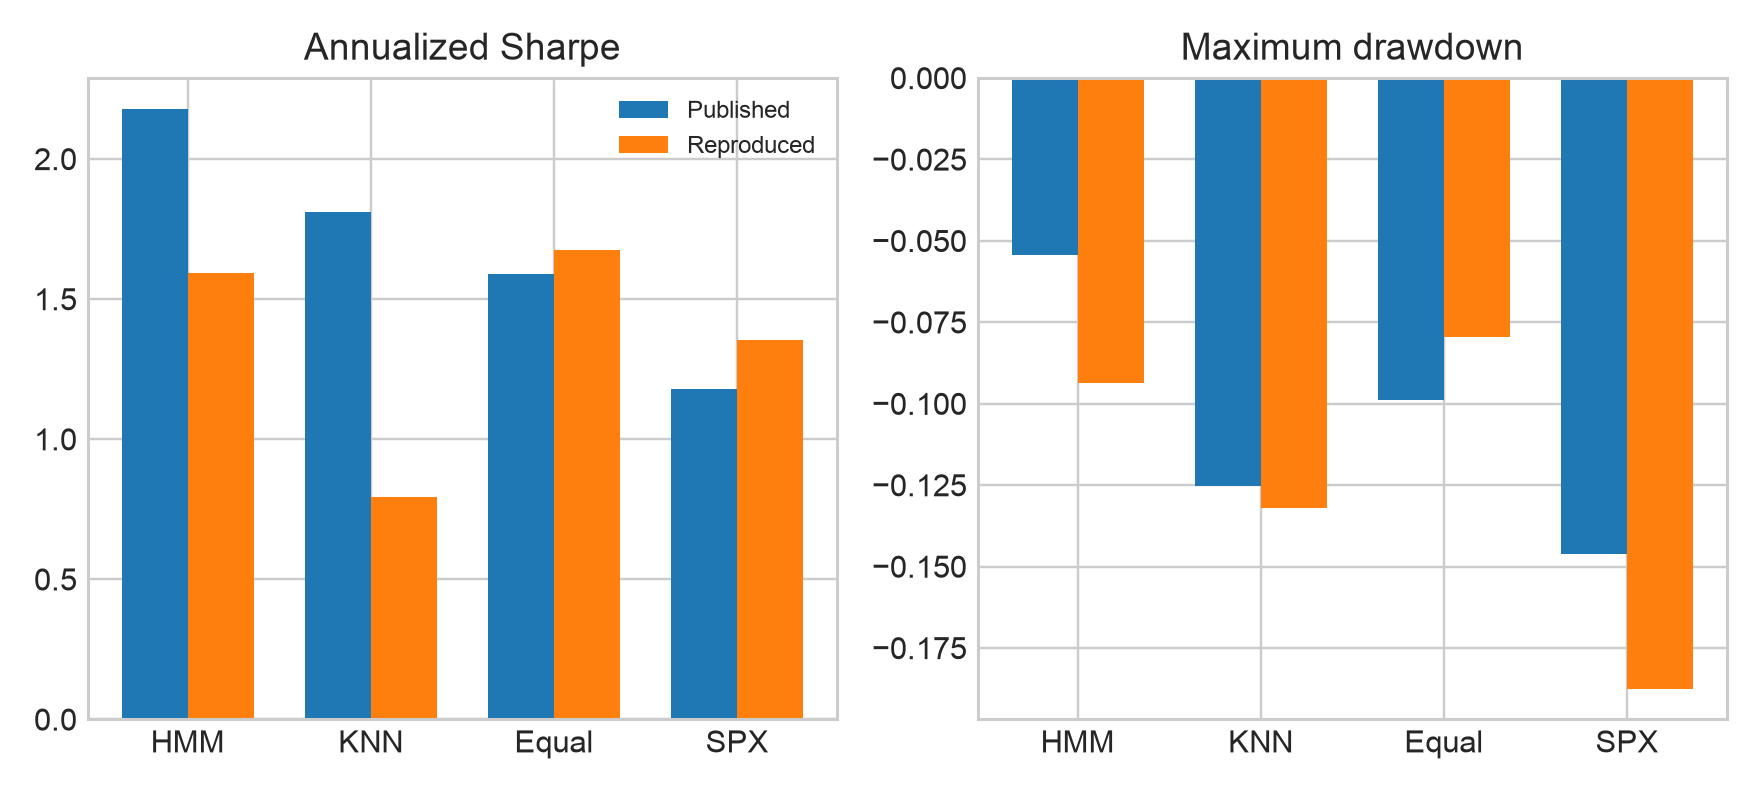
\includegraphics[width=0.88\linewidth]{published_vs_reproduced.png}
\caption{Published targets and independently reproduced outcomes. The gap is not a confidence interval; it is a discrepancy between two implementations whose specifications are not identical because the target implementation is undisclosed.}
\label{fig:published-reproduced}
\end{figure}

\subsection{Wealth paths and the 2025 drawdown}

Figure~\ref{fig:wealth} shows compounded gross wealth. The HMM participates in the broad risk-asset advance but does not reproduce the exceptionally smooth path shown in the target paper. It falls less than SPY during the 2025 selloff, yet its full-sample drawdown remains larger than equal weight's. The result supports a diversification effect, but not a unique regime-model advantage.

\begin{figure}[H]
\centering
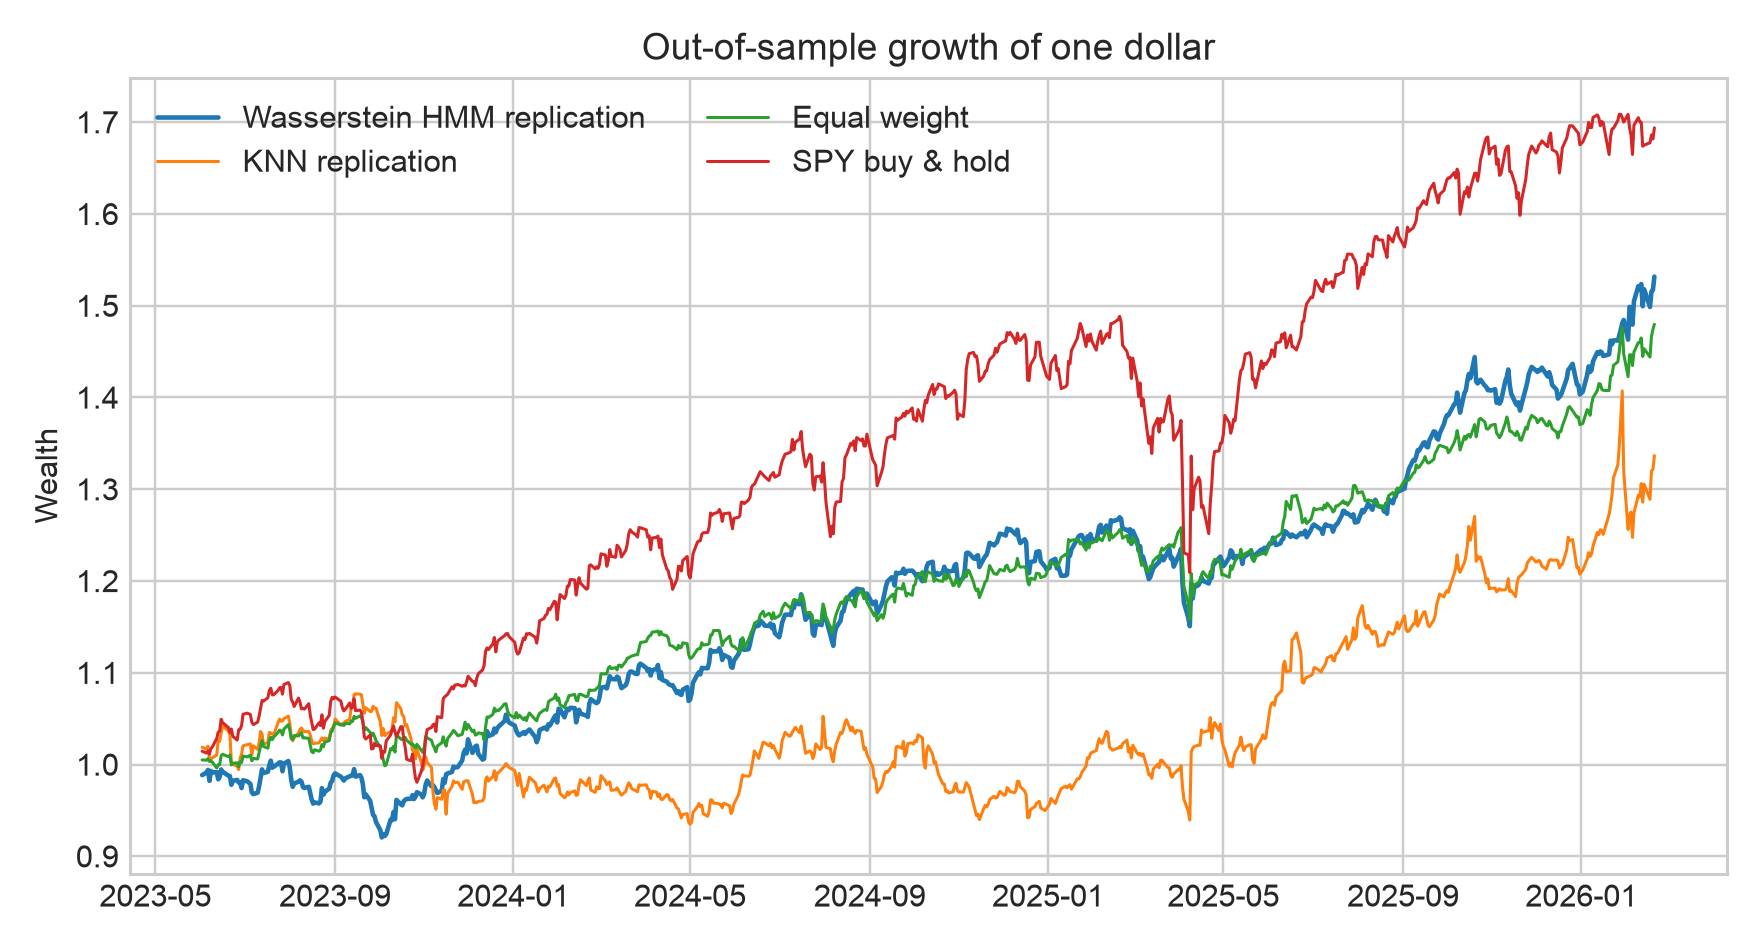
\includegraphics[width=0.94\linewidth]{cumulative_performance.png}
\caption{Growth of one dollar over the common out-of-sample interval.}
\label{fig:wealth}
\end{figure}

\subsection{Turnover and allocation stability}

The strongest replicated finding concerns stability. Average one-way turnover is \RepHMMTurnover{} for the HMM and \RepKNNTurnover{} for KNN. Their 95th percentiles are \RepHMMTurnoverQ{} and \RepKNNTurnoverQ{}, respectively. KNN turnover is therefore \TurnoverRatio{} times the HMM value on average. The magnitude does not exactly match the published pair \PubHMMTurnover{} and \PubKNNTurnover{}, but the ordering and economic interpretation are robust.

Average HMM allocations are \AvgSPYWeight{} SPY, \AvgTLTWeight{} TLT, \AvgGLDWeight{} GLD, \AvgUSOWeight{} USO, and \AvgUUPWeight{} UUP. These averages differ materially from the target paper, further indicating that its proxy set, conditional-moment bridge, or optimizer parameters differ from ours.

\begin{figure}[H]
\centering

\includegraphics[width=0.96\linewidth]{weights_and_turnover.png}
\caption{Reproduced HMM weights and daily one-way turnover. KNN allocation changes are discontinuous, while HMM positions are piecewise persistent around refits and regime transitions.}
\label{fig:weights-turnover}
\end{figure}

\subsection{Realized-cost sensitivity}

Table~\ref{tab:costs} distinguishes an optimizer penalty from actual return deductions. At \RealizedCost{} basis points per unit turnover, HMM Sharpe declines only from \RepHMMSharpe{} to \RepHMMNetSharpe{}. KNN Sharpe falls from \RepKNNSharpe{} to \RepKNNNetSharpe{} and its maximum drawdown expands to \RepKNNNetMaxDD{}. Thus, even though the target performance ranking is not reproduced, the claim that unstable local-neighbor estimates are economically fragile under trading costs is supported.

\begin{table}[H]
\centering
\caption{Gross and net performance under explicit realized trading costs.}
\label{tab:costs}
\begin{tabular}{lrrrr}
\toprule
& Gross Sharpe & Net Sharpe & Gross total return & Net total return \\
\midrule
Wasserstein HMM & \RepHMMSharpe{} & \RepHMMNetSharpe{} & \RepHMMReturn{} & \RepHMMNetReturn{} \\
KNN & \RepKNNSharpe{} & \RepKNNNetSharpe{} & \RepKNNReturn{} & \RepKNNNetReturn{} \\
\bottomrule
\end{tabular}
\end{table}

\section{Why Exact Replication Fails}

\subsection{Underdetermined empirical specification}

The economic labels are not executable ticker identifiers. SPX could mean an index without dividends, SPY with dividends, a futures series, or a volatility-targeted sleeve. BOND could refer to duration exposures ranging from aggregate bonds to long Treasuries. Similar ambiguity applies to OIL and USD. These choices alter both the conditioning features and realized portfolio returns.

The paper also omits candidate HMM orders, covariance type, feature standardization, validation length, template initialization, smoothing rate, risk aversion, turnover penalty, maximum weight, random seed, and convergence controls. These are not secondary software details: they jointly determine regime persistence, expected returns, and trading intensity.

\subsection{Causal timing ambiguity}

The paper defines \(x_t\) using \(r_t\), states that all features at \(t\) use information only through \(t-1\), and then realizes \(w_t^\top r_t\) in pseudocode. Those statements cannot all hold unless \(r_t\) is relabeled as a lagged return. We choose the conservative interpretation in Equation~\eqref{eq:features}. A same-session implementation would introduce look-ahead and could materially inflate performance.

\subsection{Dimension mismatch in conditional moments}

HMM emissions live in \(\mathbb{R}^{3N}\), while portfolio weights live in \(\mathbb{R}^{N}\). The source equations use the Gaussian component parameters directly as portfolio moments without defining how feature moments become asset-return moments. Equation~\eqref{eq:returnmoments} is our explicit solution, but alternative causal mappings are possible and can produce different allocations.

\subsection{Conflicting source artifacts}

The submitted arXiv bundle includes an older table with different HMM results and a newer table labeled in comments as ``Commercial V2.0 Parametric,'' while the same image files are retained. The bundle contains no executable source or data snapshot. Consequently, neither version identifies a unique computational experiment.

\subsection{Benchmark non-reconciliation}

The target paper reports SPX Sharpe \PubSPXSharpe{} and maximum drawdown \PubSPXMaxDD{}. On the apparent test interval, standard adjusted-close calculations for SPY produce \RepSPXSharpe{} and \RepSPXMaxDD{}. Since a passive benchmark requires no HMM assumptions, this disagreement is especially informative: the return series or metric conventions must differ before any model-level comparison begins.

\section{Interpretation}

The evidence supports a narrower claim than the target paper advances. Structured latent-state inference and template persistence can reduce allocation discontinuity relative to an unsmoothed KNN estimator. This result is both statistically visible and economically important after explicit trading costs.

The evidence does not establish that the Wasserstein HMM dominates naive diversification. In this reproduction, equal weight has higher Sharpe, lower drawdown, and a similarly smooth wealth path. The HMM's complexity is therefore not justified by the observed performance advantage alone. Its remaining value lies in conditional attribution, adaptive exposures, and the possibility that better-specified templates or assets generalize outside this sample.

The KNN comparison should also be interpreted carefully. An unsmoothed nearest-neighbor estimator changes its neighborhood discontinuously and is almost designed to destabilize a sensitive optimizer. Kernel weighting, neighbor persistence, regularized expected returns, or a no-trade region could substantially improve that baseline. The experiment demonstrates a weakness of this KNN construction, not a universal superiority of parametric regime models.

\section{Limitations}

This reproduction is intentionally faithful to the published architecture, but several limitations remain. First, the ETF mapping is inferred. Second, hyperparameters are reasonable defaults rather than recovered author settings. Third, repeated model selection and template updating create researcher degrees of freedom that are not summarized by a single backtest. Fourth, the sample contains only \OOSObs{} out-of-sample sessions and one prominent equity drawdown. Fifth, no multiple-testing adjustment, deflated Sharpe ratio, or independent second market is used. Finally, template anchoring may delay adaptation during a genuine structural break; stable labels are not necessarily correct labels.

\section{Conclusion}

We successfully reproduce the architecture of a causal Wasserstein-HMM allocator, including predictive order selection, persistent Gaussian templates, posterior-weighted asset moments, and transaction-penalized optimization. We do not reproduce the paper's headline numerical claims. The independent HMM reaches Sharpe \RepHMMSharpe{} and maximum drawdown \RepHMMMaxDD{}, while equal weight reaches Sharpe \RepEqualSharpe{} and maximum drawdown \RepEqualMaxDD{}.

The robust result is implementation stability: the HMM trades far less than KNN and retains most of its gross performance after explicit costs. The non-robust result is superior risk-adjusted performance over passive diversification. Without code, data, and a complete parameter manifest, the published Sharpe of \PubHMMSharpe{} should be treated as an unverified result rather than a reproducible benchmark.

\section*{Reproducibility Statement}

The implementation, cached price panel, daily weights, daily returns, configuration, figures, and machine-readable result file accompany this paper. Every empirical value in the prose and tables is generated from the result file through \texttt{numbers.tex}; values are not manually transcribed. The test suite includes a future-price perturbation check for feature causality, Wasserstein metric checks, and portfolio-feasibility checks.

\section*{Disclaimer}

This document is a methodological reproduction for research purposes. It is not investment advice, a recommendation, or evidence of future returns. Backtests are sensitive to data, assumptions, costs, and implementation choices.

\appendix
\section{Algorithmic Summary}

For each out-of-sample session \(t\):
\begin{enumerate}
  \item construct \(x_t\) only from returns observed through \(t-1\);
  \item when scheduled, select HMM order on a trailing validation slice and refit on the expanding history;
  \item map fitted Gaussian emissions to persistent templates by Equation~\eqref{eq:wasserstein};
  \item filter the current template probability vector;
  \item aggregate template-conditioned return moments by Equation~\eqref{eq:mixture};
  \item solve Equation~\eqref{eq:mvo}; and
  \item record the target weights, turnover, and session-\(t\) return.
\end{enumerate}

\section{Reproducibility Checklist}

\begin{tabular}{p{0.58\linewidth}c}
\toprule
Item & Status \\
\midrule
No future price used in feature construction & Verified by test \\
Portfolio weights non-negative and sum to one & Verified by test \\
Published and reproduced values stored separately & Yes \\
All paper numbers generated from machine-readable results & Yes \\
Gross and realized-cost returns reported separately & Yes \\
Data source and proxy mapping disclosed & Yes \\
Random seed disclosed & Yes \\
Source paper implementation available & No \\
Exact numerical claims independently reproduced & No \\
\bottomrule
\end{tabular}

\begin{thebibliography}{99}

\bibitem{boukardagha2026}
A. Boukardagha.
\newblock Explainable Regime Aware Investing.
\newblock \emph{arXiv preprint arXiv:2603.04441}, 2026.

\bibitem{hamilton1989}
J. D. Hamilton.
\newblock A new approach to the economic analysis of nonstationary time series and the business cycle.
\newblock \emph{Econometrica}, 57(2):357--384, 1989.

\bibitem{rabiner1989}
L. R. Rabiner.
\newblock A tutorial on hidden Markov models and selected applications in speech recognition.
\newblock \emph{Proceedings of the IEEE}, 77(2):257--286, 1989.

\bibitem{ledoitwolf2004}
O. Ledoit and M. Wolf.
\newblock A well-conditioned estimator for large-dimensional covariance matrices.
\newblock \emph{Journal of Multivariate Analysis}, 88(2):365--411, 2004.

\bibitem{demiguel2009}
V. DeMiguel, L. Garlappi, and R. Uppal.
\newblock Optimal versus naive diversification: How inefficient is the 1/N portfolio strategy?
\newblock \emph{Review of Financial Studies}, 22(5):1915--1953, 2009.

\bibitem{peyre2019}
G. Peyr\'e and M. Cuturi.
\newblock Computational optimal transport.
\newblock \emph{Foundations and Trends in Machine Learning}, 11(5--6):355--607, 2019.

\bibitem{stephens2000}
M. Stephens.
\newblock Dealing with label switching in mixture models.
\newblock \emph{Journal of the Royal Statistical Society: Series B}, 62(4):795--809, 2000.

\end{thebibliography}

\end{document}
